\documentclass[9pt]{article}
\usepackage{geometry}
\geometry{a4paper}
\usepackage{graphicx}
\usepackage{float}
\usepackage{tikz}
\usepackage{hyperref}
\usetikzlibrary{mindmap,shadows}
\linespread{1.2}

\begin{document}
%----------------------------------------------------------------------------------------
%	TITLE PAGE
%----------------------------------------------------------------------------------------

\begin{titlepage}

\newcommand{\HRule}{\rule{\linewidth}{0.5mm}}
\center
\textsc{\LARGE University of Southampton}\\[1.5cm]
\textsc{\Large Msc Cyber Security}\\[0.5cm]
\textsc{\large Project Preparation}\\[0.5cm]
\HRule \\[0.4cm]
{ \huge \bfseries Risk profiling using NLP }\\[0.4cm]
\HRule \\[1.5cm]

\begin{minipage}{0.4\textwidth}
\begin{flushleft} \large
\emph{Author:}\\
Gerard \textsc{Tio Nogueras}
\end{flushleft}
\end{minipage}
~
\begin{minipage}{0.4\textwidth}
\begin{flushright} \large
\emph{Supervisor:} \\
Dr. Sylvain \textsc{Frey}
\end{flushright}
\end{minipage}\\[4cm]

%{\large \today}\\[3cm]
%\includegraphics{Logo}\\[1cm] % Include a department/university logo - this will require the graphicx package

\vfill
\end{titlepage}
%----------------------------------------------------------------------------------------
%	INTRODUCTION
%----------------------------------------------------------------------------------------
\section{What is the reader supposed to learn?}
\begin{itemize}
\item main people/technologies in the field (check for a bible and standard technologies/libraries)
\item recent major advances and discoveries (check for latest updated technology)
\item gaps in the research (nlp sentiment alaysis doesn't have a risk based decision section or a risk assessment modelling)
\item current debates (might not come into our review)
\item where the subject might go next (explain the different obj of the project: present the paper with new evidences, expand the game, use the game in companies as training but also as an evaluation of the risk based decisions taken by the employees)
\end{itemize}

\section{Our job}
Provide an insight by taking the knowledge gained and explain the subject of the review to the reader.

\section{Our contribution}
Cover the major players in the field and give your critical opinion about these players regarding the context of the subject.(matrix)

\section{Importance of Critical thinking}
Be very critical of the references used in the review. Be critical when reading the and their results. Not only their results but their methods are correct.\\\\
This is important when finding disagreements in different references and then talk about debate in the field.
\section{The matrix}
To present the references used and their content; as well as the different possibilities that exist for a specific technology/field. \\ To do so we create a matrix:
\begin{itemize}
\item FEATURES(x) and REFERENCES(y)
\item POSSIBILITIES(x) and FEATURES(y)
\end{itemize}
Then you use these matrix to present your review. You can do so following to strategies:
\begin{itemize}
\item chronological: present the technologies or references by chronological order.
\item Feature: present the different features and for each feature present which references talk about it and the differences found there.
\end{itemize}
IMPORTANT: 
Technology reviews are best done by taking each reference and exploring the key features. You can use a scoring for each feature to provide a ranking.\\
\textbf{Surveys of a discipline with a strong narrative of the discipline itself are best done by talking about each feature in turn with all relevant references.}\\\\
ADD THIS TABLE AT THE END TO SUMMARIZE THE REVIEW.

\section{List of features with concerned papers}

\section{Idea}
List all the interesting references, highlight the top 10 to create a state of the art for my project and give access to abstracts of the entire list of references used.
\\\\
key search words: "profiling" "risk assessment" "cyber security" "summarizing" "report" "risk-based decision" "decision making" "risk analysis" "perception modelling" "risk perception modelling" "opinion" "emotion" "sentiment"
\\\\
NEXT STEP: Commencer à écrire qu'est-ce que NLP, à quoi ça sert, et pourquoi on veut l'utiliser dans ce cas précis ça aidera à focaliser la recherche / lecture de nouveau papiers et identifier des angles morts dans l'état de l'art, tel que NLP for risk perception.
\\\\
Possible final subject: Cyber security Risk perception using NLP

\section{Mindmap}

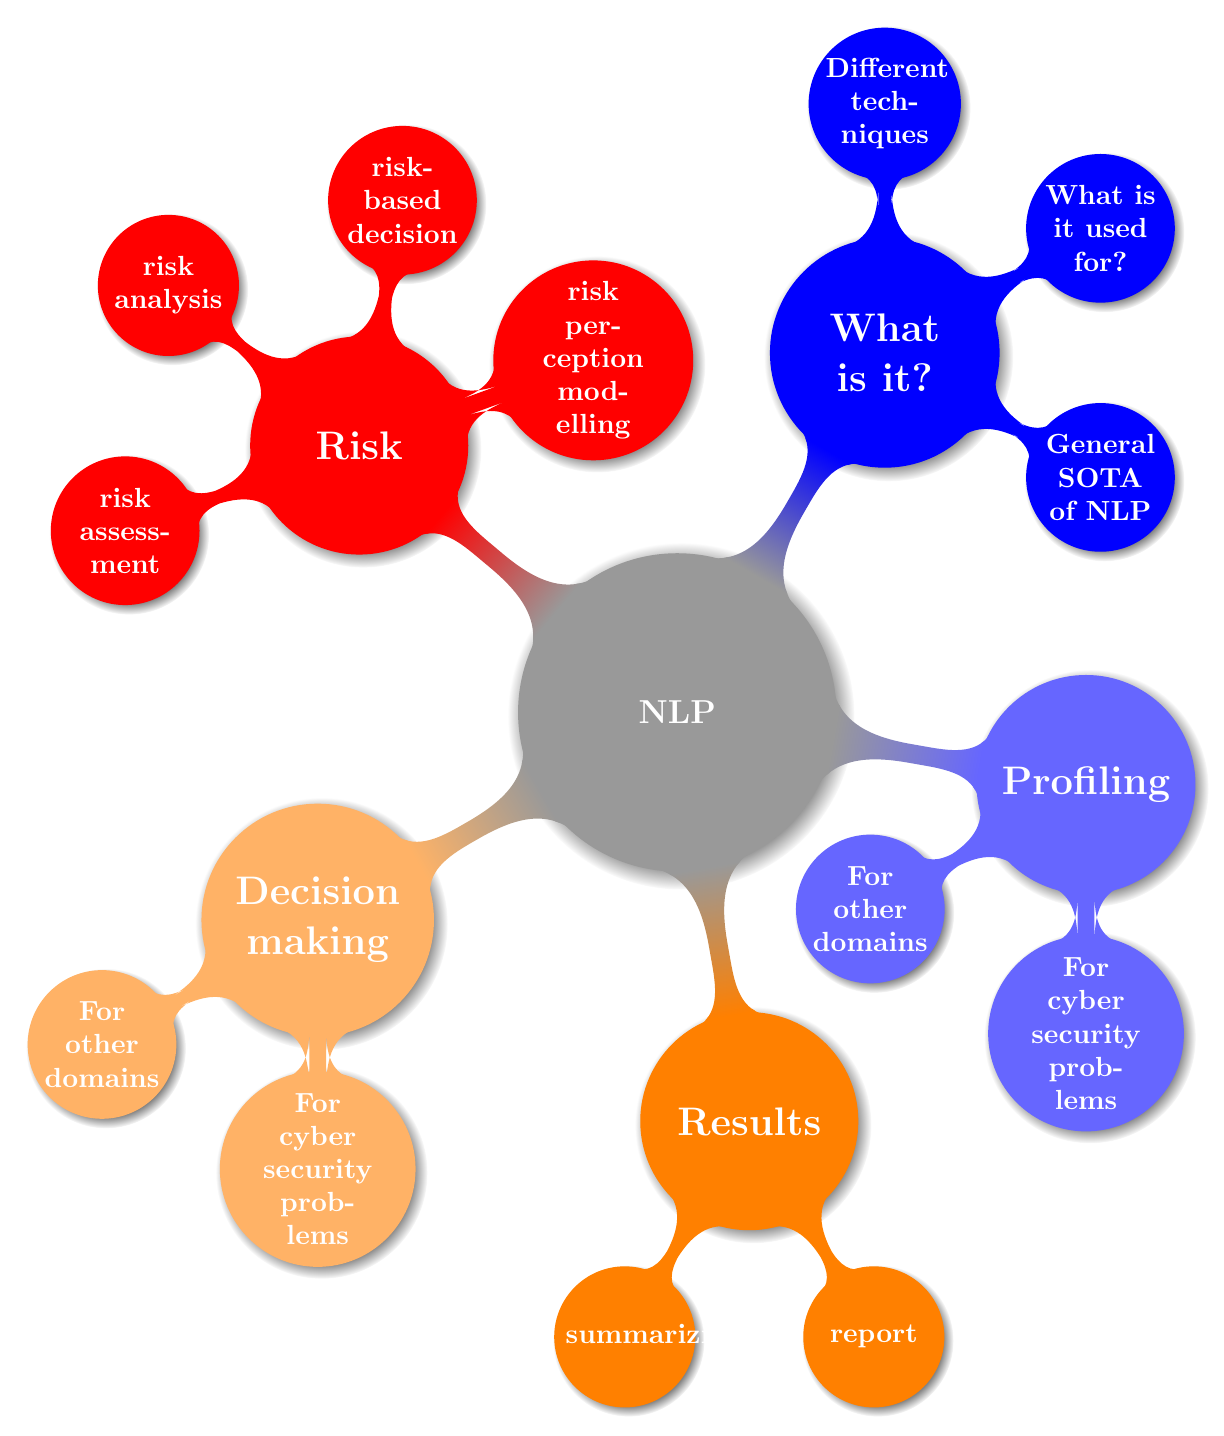
\begin{tikzpicture}[ every annotation/.style = {draw,
                     fill = white, font = \Large}]
  \path[mindmap,concept color=black!40,text=white,
    every node/.style={concept,circular drop shadow},
    root/.style    = {concept color=black!40,
      font=\large\bfseries,text width=10em},
    level 1 concept/.append style={font=\Large\bfseries,
      sibling angle=70,text width=7.7em,
    level distance=15em,inner sep=0pt},
    level 2 concept/.append style={font=\bfseries,level distance=9em},
  ]
  node[root] {NLP} [clockwise from=60]
    child[concept color=blue] {
      node {What is it?} [clockwise from=90]
      	child { node {Different techniques}}
      	child { node {What is it used for?}}
      	child { node {General SOTA of NLP}}
    }
    child[concept color=blue!60] {
      node {Profiling} [clockwise from=270]
      	child { node {For cyber security problems}}
      	child { node {For other domains}}
    }
    child[concept color=orange] {
      node {Results} [clockwise from=300]
      	child { node {report}}
      	child { node {summarizing}}
    }
    child[concept color=orange!60] {
      node {Decision making} [clockwise from=270]
      	child { node {For cyber security problems}}
      	child { node {For other domains}}
    }
    child[concept color=red, level distance=15em] {
      node {Risk} [clockwise from=200]
      	child { node {risk assessment}}
      	child { node {risk analysis}}
      	child { node {risk-based decision}}
      	child { node {risk perception modelling}}
    }
    ;
\end{tikzpicture}

%----------------------------------------------------------------------------------------
%	CONTENT
%----------------------------------------------------------------------------------------
\section{Intro}
%Commencer à écrire qu'est-ce que NLP, à quoi ça sert, et pourquoi on veut l'utiliser dans ce cas précis ça aidera à focaliser la recherche / lecture de nouveau papiers et identifier des angles morts dans l'état de l'art, tel que NLP for risk perception.
\subsection{Where does this research come from}
"Stakeholders’ in security decisions play a fundamental role in determining security requirements, yet, little is currently understood about how different stakeholder groups within an organisation approach security and the drivers and tacit biases underpinning their decisions"\cite{DnD}. To have a better understanding about this subject my supervisor Dr. Sylvain \textsc{Frey} created a board game that simulates these interactions. 
The problem he/his team encountered when proposing their results to the main cyber security conferences (not sure of the term to use here) is that their results can not be accepted because of the low amount of games played. 
Therefore we are trying to find other ways to support their results.
\subsection{What is NLP?}
Natural processing language,{summarize wiki and what is interesting to us} 

\subsection{Why are we interested in NLP?}
We possess scripted recordings of 12 game-plays. Using NLP we hope to achieve a report of the interactions by profiling the players and their risk-based decisions. We wish to visualize the starting state of the players, their adaptations, their knowledge, the interactions with a "champion", how risk is taken into account, how different backgrounds affect the decision-making process and {ADD HERE MORE RELEVANT GOALS}
+ {present some papers that will be the base ground of our research}

\subsection{What do we hope to achieve?}
The final goal of this project/research is to support the results found previously and additionally to be able to create reports with constructive criticism of the flaws of the players methodology and the approaches taken during the game to enhance the risk based decisions of the different entities of the company.
\\\\
Another aspect that we hope to achieve is to create a starting ground for future research on risk-based profiling for cyber security decisions. Because right now there is a lot of research done on medical risk but not on cyber security risk decisions.

\section{TOP 10 research papers}
\begin{itemize}
\item The Good, the Bad and the Ugly: A Study of Security Decisions in a Cyber-Physical Systems Game \cite{DnD}
\item A COMPARATIVE STUDY OF SENTIMENT ANALYSIS TECHNIQUES \cite{sentiment analysis}
\end{itemize}
\section{TOP 50 research papers}
\begin{itemize}
\item The Good, the Bad and the Ugly: A Study of Security Decisions in a Cyber-Physical Systems Game \cite{DnD}
\item Natural Language Processing in Accounting, Auditing and Finance: A Synthesis of the Literature with a Roadmap for Future Research\cite{nlpfinance}
\item The role of behavioral research and profiling in malicious cyber insider investigations\cite{nlpinvestigation}
\item Cyber security risk assessment for SCADA and DCS networks \cite{risk assessment}
\item Profiling Enterprise Risks in Large Computer Companies Using the Leximancer Software Tool\cite{profiling risk}
\item The challenges of automatic summarization \cite{summarization}
\item Mining and summarizing customer reviews \cite{mining summarizing}
\item Natural language processing for information retrieval \cite{nlp info}
\item Sentiment analysis: capturing favorability using natural language processing \cite{nlpsentiment}
\item Ontology-based parser for natural language processing \cite{nlpparser}
\item Systems for natural language processing of sentence based queries \cite{nlpqueries}
\item Automated Product Profiling through NLP \cite{product profiling}
\item Natural Language Processing \cite{nlp2}
\item Profiling Academic Research on Digital Games Using Text Mining Tools \cite{games profiling}
\item Semantic Web Mining: State of the art and future directions \cite{web mining}
\item Social tagging in recommender systems: a survey of the state-of-the-art and possible extensions \cite{social tagging}
\item Deep Learning for Natural Language Processing (without Magic) \cite{tuto}
\item Stanford CoreNLP \cite{program}
\item Natural Language Processing: State of the Art and Prospects for Significant Progress, A workshop sponsored by the National Library of Medicine \cite{nlp sota medecine}
\item The linguistic approach to the natural language requirements quality: benefit of the use of an automatic tool \cite{nlp methodology}
\item Natural language processing: an introduction \cite{advanced tuto}
\item Pattern Recognition and Natural Language Processing: State of the Art \cite{nlp sota}
\item Semantic Analysis for Monitoring Insider Threats \cite{inside threats}
\item Learning to Connect Language and Perception \cite{language and perception}
\item Precisiated Natural Language \cite{pnl}
\item A COMPARATIVE STUDY OF SENTIMENT ANALYSIS TECHNIQUES \cite{sentiment analysis}
\item Jumping NLP Curves: A Review of Natural Language Processing Research \cite{review nlp}
\item NLTK: the Natural Language Toolkit \cite{nltk}
\item Identifying Expressions of Opinion in Context \cite{opinion}
\item Sentiment analyzer: extracting sentiments about a given topic using natural language processing techniques \cite{sentiment analyzer}
\item OpinionFinder: a system for subjectivity analysis \cite{opinion finder}
\item Annotating Expressions of Opinions and Emotions in Language \cite{expressions opinion}
\item Thumbs  up?  sentiment classification using machine learning techniques \cite{thumbs}
\item Direction-based text interpretation as an information access refinement \cite{direction}
\item On the computation of point of view \cite{computation}
\
\end{itemize}


Possible interesting papers: \\
\textbf{Sentiment classifiers:} \\



S. Das and M. Chen.   Yahoo! for amazon: Extracting market sentiment from stock message boards. In Proc. of the 8th APFA, 2001. \url{http://citeseer.ist.psu.edu/viewdoc/summary?doi=10.1.1.202.6418}\\
R. M. Tong.  An operational system for detecting and track-
ing opinions in on-line discussion.   In SIGIR Workshop on Operational Text Classification, 2001.\\
\textbf{Affect analysis:} \\
P. Subasic  and  A.  Huettner.   Affect  analysis  of  text  using fuzzy semantic typing. IEEE Trans. on Fuzzy Systems, Special Issue, Aug., 2001.\\
C. Whissell.  The dictionary of affect in language. Emotion: Theory, Research, and Experience, pages 113–131.\\
automatic survey analysis:\\
H. Li and K. Yamanishi. Mining from open answers in questionnaire data. In Proc. of the 7th ACM SIGKDD Conf. , 2001.\\
\textbf{opinion extraction: }\\
S. Morinaga, K. Yamanishi, K. Teteishi, and T. Fukushima. Mining product reputations on the web.  In Proc. of the 8th ACM SIGKDD Conf. , 2002.\\
\textbf{Recommender systems: }\\
L. Terveen, W. Hill, B. Amento, D. McDonald, and J. Creter. PHOAKS: A system for sharing recommendations. CACM, 40(3):59–62, 1997.\\
\section{Non-research information}
\begin{itemize}
\item OpenDNS Uses Natural Language Processing to Detect APTs \cite{opendns}
\item Using Natural Language Processing to Identify Malicious Domains
\item BASICS OF NLP \cite{nlp}
\item NLP Ideas \cite{ideas}
\item NLP wiki \cite{wiki}
\item SOTA nlp 2015 \cite{reddit sota}
\item NLP english \cite{eng wiki}
\end{itemize}
%----------------------------------------------------------------------------------------
%	BIBLIOGRAPHY
%----------------------------------------------------------------------------------------
\newpage
\begin{thebibliography}{99}
\bibitem {DnD} Sylvain Frey, Awais Rashid, Pauline Anthonysamy, Maria Pinto-Albuquerque, and Syed Asad Naqvi. 2016.  The Good, the Bad and the Ugly: A Study of Security Decisions in a Cyber-Physical Systems Game.

%\bibitem {nlpparser} \url{https://www.google.com/patents/US7027974}

%\bibitem {nlpqueries} \url{https://www.google.com/patents/US20100005081}

\bibitem {product profiling} \url{https://nlp.stanford.edu/courses/cs224n/2011/reports/jihohan-gogo9th.pdf}

%\bibitem {nlp2} \url{https://www.cl.cam.ac.uk/teaching/2002/NatLangProc/revised.pdf}

%\bibitem {games profiling} \url{http://homes.lmc.gatech.edu/~cpearce3/DiGRA07/Proceedings/094.pdf}

%\bibitem {web mining} \url{http://www.sciencedirect.com/science/article/pii/S1570826806000084}

%\bibitem {social tagging} \url{http://link.springer.com/article/10.1007/s10462-009-9153-2}

%\bibitem {ideas} \url{http://datascience.stackexchange.com/questions/2268/what-is-the-state-of-the-art-in-the-field-of-nlp}

%\bibitem {wiki} \url{https://fr.wikipedia.org/wiki/Traitement_automatique_du_langage_naturel}

%\bibitem {eng wiki} \url{https://en.wikipedia.org/wiki/Natural_language_processing}

%\bibitem {nlpsentiment} \url{http://dl.acm.org/citation.cfm?id=945658}

%\bibitem {nlpinfo} \url{http://dl.acm.org/citation.cfm?id=234210}

%\bibitem {mining summarizing} \url{http://dl.acm.org/citation.cfm?id=1014073}

%\bibitem {opendns} \url{http://www.securityweek.com/opendns-uses-natural-language-processing-detect-apts}

%\bibitem {opendns2} \url{https://securityintelligence.com/news/using-natural-language-processing-identify-malicious-domains/}

%\bibitem {nlpfinance} \url{http://onlinelibrary.wiley.com/doi/10.1002/isaf.1386/full}

%\bibitem {nlpinvestigation} \url{http://www.sciencedirect.com/science/article/pii/S1742287606000090}

%\bibitem {nlp} \url{http://stp.lingfil.uu.se/~santinim/ml/2014/JurafskyMartinSpeechAndLanguageProcessing2ed_draft\%202007.pdf} \url{https://www.cs.colorado.edu/~martin/SLP/Updates/1.pdf}

%\bibitem {risk assessment} \url{http://www.sciencedirect.com/science/article/pii/S0019057807000754}

\bibitem {profiling risk} \url{http://link.springer.com/article/10.1057/palgrave.rm.8250030}

\bibitem {summarization} \url{http://ieeexplore.ieee.org/abstract/document/881692/}

\bibitem {tuto} \url{https://nlp.stanford.edu/courses/NAACL2013/} $+$ \url{http://nlp.stanford.edu/~socherr/DeepLearning-ACL2012-tutorial.pdf}

\bibitem {program} \url{http://stanfordnlp.github.io/CoreNLP/} $+$ \url{http://nlp.stanford.edu/pubs/StanfordCoreNlp2014.pdf}

\bibitem {nlp sota medecine} \url{https://www.researchgate.net/publication/243966799_Natural_Language_Processing_State_of_the_Art_and_Prospects_for_Significant_Progress_A_workshop_sponsored_by_the_National_Library_of_Medicine}

\bibitem {reddit sota} \url{https://www.reddit.com/r/MachineLearning/comments/4020ek/state_of_the_art_dec2015_natural_language/}

\bibitem {nlp methodology} \url{http://ieeexplore.ieee.org/abstract/document/992662/}

\bibitem {advanced tuto} \url{https://www.ncbi.nlm.nih.gov/pmc/articles/PMC3168328/}

\bibitem {nlp sota} \url{http://www.temjournal.com/content/52/TemJournalMay2016_236_240.pdf}

\bibitem {inside threats} \url{http://link.springer.com/chapter/10.1007/978-3-540-25952-7_40}

\bibitem {language and perception} \url{http://www.aaai.org/Papers/AAAI/2008/AAAI08-271.pdf}

\bibitem {pnl} \url{http://www.aaai.org/ojs/index.php/aimagazine/article/view/1778}

\bibitem {sentiment analysis} \url{https://pdfs.semanticscholar.org/3f10/b006bab60c7f363bc03e72ad405d264b8d42.pdf}

\bibitem {review nlp} \url{http://ieeexplore.ieee.org/abstract/document/6786458/?part=1}

\bibitem {nltk} \url{http://dl.acm.org/citation.cfm?id=1118117}

\bibitem {opinion} \url{http://www.aaai.org/Papers/IJCAI/2007/IJCAI07-431.pdf}

\bibitem {sentiment analyzer} \url{http://ieeexplore.ieee.org/abstract/document/1250949/} \url{http://ieeexplore.ieee.org/stamp/stamp.jsp?arnumber=1250949}

\bibitem {opinion finder} \url{http://dl.acm.org/citation.cfm?id=1225751}

\bibitem {expressions opinion} \url{http://link.springer.com/article/10.1007\%2Fs10579-005-7880-9?LI=true}

\bibitem {thumbs} B. Pang, L. Lee, and  S. Vaithyanathan.   Thumbs  up?  sentiment classification using machine learning techniques.  In Proc. of the 2002 ACL EMNLP Conf. , pages 79–86, 2002. \url{https://www.cs.cornell.edu/home/llee/papers/sentiment.pdf}\\

\bibitem {direction} M. Hearst. Direction-based text interpretation as an informa-tion access refinement. Text-Based Intelligent Systems, 1992. \url{http://citeseerx.ist.psu.edu/viewdoc/download;jsessionid=2037E600F4275AC38D0DCDE1010C71B3?doi=10.1.1.40.9124&rep=rep1&type=pdf} or \url{http://citeseerx.ist.psu.edu/viewdoc/summary?doi=10.1.1.40.9124}\\

\bibitem {computation} W. Sack.  On the computation of point of view.  In Proc. of the 12th AAAI Conf., 1994. \url{http://www.aaai.org/Papers/AAAI/1994/AAAI94-282.pdf}
\end{thebibliography}
\end{document}